% This is the Reed College LaTeX thesis template. Most of the work
% template. Later comments etc. by Ben Salzberg (BTS). Additional
% restructuring and APA support by Jess Youngberg (JY).
% Your comments and suggestions are more than welcome; please email
% them to cus@reed.edu
%
% See http://web.reed.edu/cis/help/latex.html for help. There are a
% great bunch of help pages there, with notes on
% getting started, bibtex, etc. Go there and read it if you're not
% already familiar with LaTeX.
%
% Any line that starts with a percent symbol is a comment.
% They won't show up in the document, and are useful for notes
% to yourself and explaining commands.
% Commenting also removes a line from the document;
% very handy for troubleshooting problems. -BTS

% As far as I know, this follows the requirements laid out in
% the 2002-2003 Senior Handbook. Ask a librarian to check the
% document before binding. -SN

%%
%% Preamble
%%
% \documentclass{<something>} must begin each LaTeX document
\documentclass[12pt,twoside]{reedthesis}
% Packages are extensions to the basic LaTeX functions. Whatever you
% want to typeset, there is probably a package out there for it.
% Chemistry (chemtex), screenplays, you name it.
% Check out CTAN to see: http://www.ctan.org/
%%
\usepackage{graphicx,latexsym}
\usepackage{amssymb,amsthm,amsmath}
\usepackage{longtable,booktabs,setspace}
\usepackage{chemarr} %% Useful for one reaction arrow, useless if you're not a chem major

% Modified by CII
\usepackage[hyphens]{url}
\usepackage{hyperref}

\usepackage{rotating}

% Added by CII
%\usepackage{hanging}
%\usepackage{natbib}

\usepackage[backend=bibtex, sorting=none, style=authoryear]{biblatex}
%\DeclareLanguageMapping{american}{american-apa}
\addbibresource{thesis}
% \bibliographystyle{APA/apa-good}  % or
%\bibliography{thesis}


% Comment out the natbib line above and uncomment the following two lines to use the new
% biblatex-chicago style, for Chicago A. Also make some changes at the end where the
% bibliography is included.

%\usepackage[backend=bibtex]{biblatex-chicago}
%\addbibresource{thesis}
%\bibliography{thesis}

% \usepackage{times} % other fonts are available like times, bookman, charter, palatino

\title{My Final College Paper}
%\author{Your R. Name}
\author{Your R. Name}
% The month and year that you submit your FINAL draft TO THE LIBRARY (May or December)
\date{May 20xx}
\division{Mathematics and Natural Sciences}
\advisor{Advisor F. Name}
%If you have two advisors for some reason, you can use the following
%\altadvisor{Your Other Advisor}
%%% Remember to use the correct department!
\department{Mathematics}
% if you're writing a thesis in an interdisciplinary major,
% uncomment the line below and change the text as appropriate.
% check the Senior Handbook if unsure.
%\thedivisionof{The Established Interdisciplinary Committee for}
% if you want the approval page to say "Approved for the Committee",
% uncomment the next line
%\approvedforthe{Committee}

\setlength{\parskip}{0pt}
%%
%% End Preamble
%%
%

% Below added by CII

\renewcommand{\contentsname}{Table of Contents}
%\renewcommand{\bibname}{References}
\DefineBibliographyStrings{english}{%
  references = {Works Cited},% replace "references" with "bibliography"  for `book`/`report`
}

\providecommand{\tightlist}{%
  \setlength{\itemsep}{0pt}\setlength{\parskip}{0pt}}

\Acknowledgements{
I want to thank a few people. Not changing?
}

\Dedication{
You can have a dedication here if you wish.
}

\Preface{
This is an example of a thesis setup to use the reed thesis document
class.
}

\Abstract{
The preface pretty much says it all.
}

\begin{document}

      \maketitle
  
  \frontmatter % this stuff will be roman-numbered
  \pagestyle{empty} % this removes page numbers from the frontmatter

      \begin{acknowledgements}
      I want to thank a few people. Not changing?
    \end{acknowledgements}
  
      \begin{preface}
      This is an example of a thesis setup to use the reed thesis document
      class.
    \end{preface}
  
  % Add table of abbreviations?

    {
    \hypersetup{linkcolor=black}
    \setcounter{tocdepth}{2}
    \tableofcontents
  }
  
      \listoftables
  
      \listoffigures
  
      \begin{abstract}
      The preface pretty much says it all.
    \end{abstract}
  
      \begin{dedication}
      The preface pretty much says it all.
    \end{dedication}
  
%  
  \mainmatter % here the regular arabic numbering starts
  \pagestyle{fancyplain} % turns page numbering back on

  \chapter*{Introduction}
  
  \addcontentsline{toc}{chapter}{Introduction}
  
  \chaptermark{Introduction} \markboth{Introduction}{Introduction}
  
  Welcome to the R Markdown thesis template. This template is based on the
  \LaTeX~template, but hopefully will provide a nicer interface for those
  that have never used \TeX~or \LaTeX~before. (You'll see \LaTeX~code here
  and there, but it won't make up a large chunk of your thesis.) Using R
  Markdown will also allow you to easily keep track of your analyses in
  \textbf{R} chunks of code, with the resulting plots and output included
  as well. The hope is this R Markdown template gets you in the habit of
  doing reproducible research, which benefits you long-term as a
  researcher, but also will greatly help anyone that is trying to
  reproduce or build onto your results down the road.
  
  Hopefully, you won't have much of a learning period to go through and
  you will reap the benefits of a nicely formatted thesis. The use of
  \LaTeX~in combination with Mardkown is more consistent than the output
  of a word processor, much less prone to corruption or crashing, and the
  resulting file is smaller than a Word file. While you may have never had
  problems using Word in the past, your thesis is going to be about twice
  as large and complex as anything you've written before, taxing Word's
  capabilities. If you're still on the fence about using R Markdown, check
  out the various tutorials available at
  \url{http://www.reed.edu/data-at-reed} or email us at
  \href{mailto:data@reed.edu}{\nolinkurl{data@reed.edu}}. After working
  with Markdown and R together for a few weeks, we are confident this will
  be your reporting style of choice going forward.
  
  \section{Why use it?}
  
  R Markdown creates a simple and straightforward way to interface with
  the beauty of \LaTeX. Packages have been written in \textbf{R} to work
  directly with \LaTeX~and its ability to do a great job of formatting
  tables and paragraphs. In addition to creating a user friendly interface
  to \LaTeX, R Markdown also allows you to read in your data, analyze it
  and visualize it using \textbf{R} functions, and also to provide the
  documentation and commentary on the results of your project. Further, it
  allows for \textbf{R} results to be passed inline to the commentary of
  your results. You'll see more on this later. Having your code and
  commentary all together in one place has a monstrosity of benefits.
  
  \section{Who should use it?}
  
  Anyone who needs to use data analysis in any form, math, tables, a lot
  of figures, complex cross-references, or who just cares about the final
  appearance of their document should use R Markdown. Of particular use
  should be anyone in the sciences, but the user-friendly nature of
  Markdown and its ability to keep track of and easily include figures,
  automatically generate a table of contents, index, references, etc.
  should make it of great benefit to nearly all seniors at Reed with their
  thesis projects.
  
  \chapter{R Markdown Basics}
  
  Here is a brief introduction into using R Markdown. Markdown is a simple
  formatting syntax for authoring HTML, PDF, and MS Word documents. For
  more details on using R Markdown see \url{http://rmarkdown.rstudio.com}.
  
  \section{Lists}\label{lists}
  
  \subsection{Unordered versus ordered}\label{unordered-versus-ordered}
  
  It's easy to create a list. It can unordered like
  
  \begin{itemize}
  \tightlist
  \item
    Item 1
  \item
    Item 2
  \item
    Item 3
  \end{itemize}
  
  or it can be ordered like
  
  \begin{enumerate}
  \def\labelenumi{\arabic{enumi}.}
  \tightlist
  \item
    Item 1
  \item
    Item 2
  \item
    Item 3
  \end{enumerate}
  
  Notice that I intentionally mislabeled Item 3 as number 4. Markdown
  automatically figures this out!
  
  To create a sublist, just indent the values a bit:
  
  \begin{enumerate}
  \def\labelenumi{\arabic{enumi}.}
  \tightlist
  \item
    Item 1
  \item
    Item 2
  \item
    Item 3
  
    \begin{itemize}
    \tightlist
    \item
      Item 3a
    \item
      Item 3b
    \end{itemize}
  \end{enumerate}
  
  \section{Line breaks}\label{line-breaks}
  
  Make sure to add white space between lines if you'd like to start a new
  paragraph. Look at what happens below if you don't:
  
  Here is the first sentence. Here is another sentence to end the
  paragraph. This should be a new paragraph.
  
  \emph{Here is the correct way:}
  
  Here is the first sentence. Here is another sentence to end the
  paragraph.
  
  This should be a new paragraph.
  
  \section{R chunks}\label{r-chunks}
  
  When you click the \textbf{Knit} button a document will be generated
  that includes both content as well as the output of any embedded R code
  chunks within the document. You can embed an R code chunk like this:
  
  \begin{CodeChunk}
  \begin{CodeInput}
  summary(cars)
  \end{CodeInput}
  \begin{CodeOutput}
       speed           dist       
   Min.   : 4.0   Min.   :  2.00  
   1st Qu.:12.0   1st Qu.: 26.00  
   Median :15.0   Median : 36.00  
   Mean   :15.4   Mean   : 42.98  
   3rd Qu.:19.0   3rd Qu.: 56.00  
   Max.   :25.0   Max.   :120.00  
  \end{CodeOutput}
  \end{CodeChunk}
  
  \section{Including Plots}\label{including-plots}
  
  You can also embed plots, for example:
  
  \begin{CodeChunk}
  
  
  \begin{center}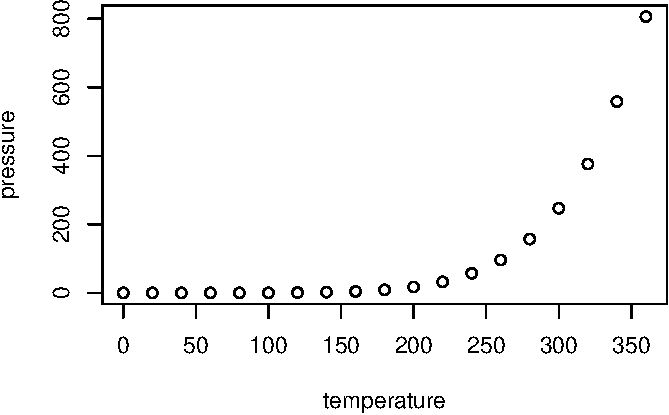
\includegraphics{skeleton_files/figure-latex/pressure-1} \end{center}
  
  \end{CodeChunk}
  
  Note that the \texttt{echo\ =\ FALSE} parameter was added to the code
  chunk to prevent printing of the R code that generated the plot. There
  are plenty of others way to add chunk options. More information is
  available at \url{http://yihui.name/knitr/options/}.
  
  \section{Inline code / Mathematics}\label{inline-code-mathematics}
  
  If you'd like to put the results of your analysis directly into your
  discussion, add inline code like this:
  
  The \texttt{cos} of \(2 \pi\) is 1.
  
  \section{Additional resources}\label{additional-resources}
  
  Markdown Cheatsheet -
  \url{https://github.com/adam-p/markdown-here/wiki/Markdown-Cheatsheet}
  
  R Markdown Reference Guide -
  \url{https://www.rstudio.com/wp-content/uploads/2015/03/rmarkdown-reference.pdf}
  
  \chapter*{Conclusion}
  
  \addcontentsline{toc}{chapter}{Conclusion}
  
  \chaptermark{Conclusion} \markboth{Conclusion}{Conclusion}
  \setcounter{chapter}{2} \setcounter{section}{0}
  
  Here's a conclusion, demonstrating the use of all that manual
  incrementing and table of contents adding that has to happen if you use
  the starred form of the chapter command. The deal is, the chapter
  command in \LaTeX~does a lot of things: it increments the chapter
  counter, it resets the section counter to zero, it puts the name of the
  chapter into the table of contents and the running headers, and probably
  some other stuff.
  
  \section{More info}
  
  And here's some other random info: the first paragraph after a chapter
  title or section head \emph{shouldn't be} indented, because indents are
  to tell the reader that you're starting a new paragraph. Since that's
  obvious after a chapter or section title, proper typesetting doesn't add
  an indent there.
  
  \appendix
  \chapter{The First Appendix} \chapter{The Second Appendix, for Fun}

  \backmatter
  \chapter{References}
  \printbibliography[heading=bibintoc, heading=none]

    % Index?

\end{document}

